% !TEX root=../root.tex

\subsection{Experiment Results}
During the flight experiments, the multirotor UAV was manually flown until the
fiducial landing marker was detected. Upon detection, the closed loop estimation
and control was given full control of the UAV. To demonstrate the ability of the
system to maintain good tracking of the landing vehicle even when the fiducial
marker is not detected for long periods of time, the fiducial marker detection
was turned off a few seconds after detection.

The results are shown in Figures~\ref{fig:hardware_gp}, \ref{fig:hardware_gv},
\ref{fig:hardware_gatt}. The fiducial landing marker is first detected at
$t$~=~20~$s$, when the plots begin. After 10 seconds, at $t$~=~30~$s$, the
fiducial marker detection is turned off for the remainder of the experiment.
Even though no measurements from the fiducial marker are used, it is clear that
the estimates of the position, velocitity, attitude and angular velocity of the
landing vehicle remain accurate and consistent for the duration of the
experiment. These accurate estimates allow
the UAV to continue to control relative to the landing vehicle, tracking closely
above the goal frame as the landing vehicle moves around the room. After the
landing vehicle has completed two full laps around the room,
at approximately $t$~=102~$s$, manual control of the UAV is resumed, ending the experiment.

A video of the flight experiment can be found at \MF{TODO make and add video}.

\begin{figure}
  \centering
  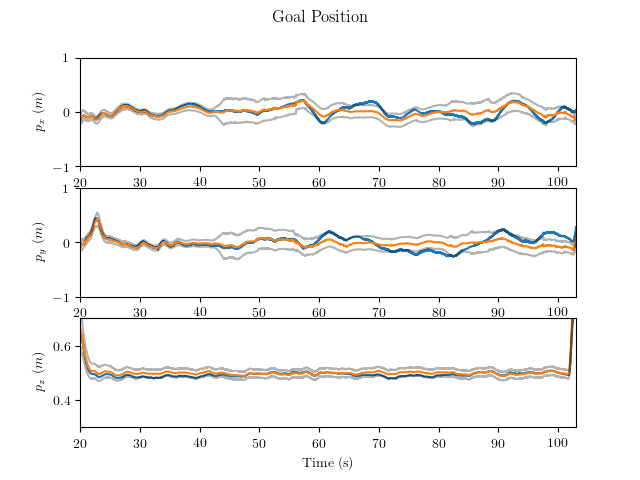
\includegraphics[scale=0.5]{plots/hardware_gp.png}
  \caption{Hardware results with the estimator using 10 visual
  landmarks. The blue line represents the true state while the orange line
  represents the estimated state. The two grey lines show a 2 $\sigma$ bound for
  the estimate based on the estimated covariance. Measurements from the fiducial
  marker are not used after $t$~=~30~$s$ to demonstrate the performance of the estimator.}
  \label{fig:hardware_gp}
\end{figure}

\begin{figure}
  \centering
  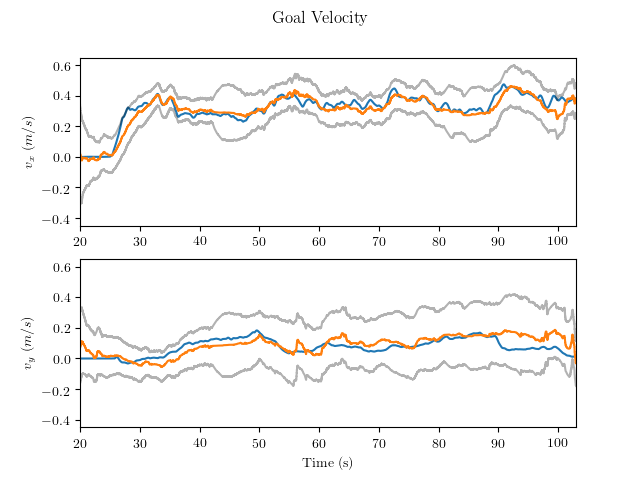
\includegraphics[scale=0.5]{plots/hardware_gv.png}
  \caption{Hardware results with the estimator using 10 visual
  landmarks. The blue line represents the true state while the orange line
  represents the estimated state. The two grey lines show a 2 $\sigma$ bound for
  the estimate based on the estimated covariance. Measurements from the fiducial
  marker are not used after $t$~=~30~$s$ to demonstrate the performance of the estimator.}
  \label{fig:hardware_gv}
\end{figure}

\begin{figure}
  \centering
  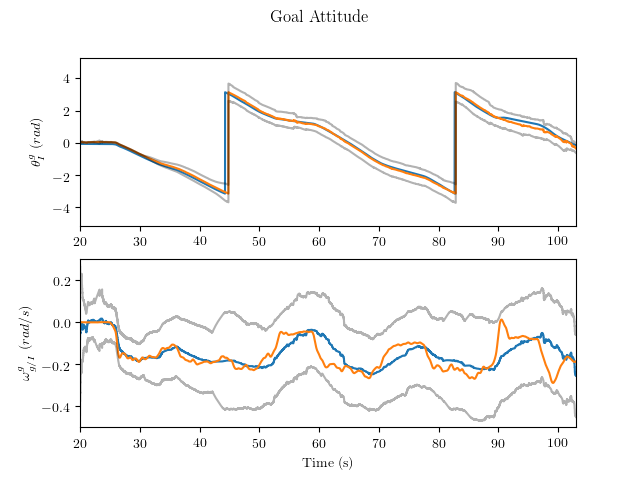
\includegraphics[scale=0.5]{plots/hardware_gatt.png}
  \caption{Hardware results with the estimator using 10 visual
  landmarks. The blue line represents the true state while the orange line
  represents the estimated state. The two grey lines show a 2 $\sigma$ bound for
  the estimate based on the estimated covariance. Measurements from the fiducial
  marker are not used after $t$~=~30~$s$ to demonstrate the performance of the estimator.}
  \label{fig:hardware_gatt}
\end{figure}
